\documentclass[11pt]{article}
\usepackage[T1]{fontenc}
\usepackage[latin1]{inputenc}
\usepackage{enumerate}
\usepackage{setspace}
\usepackage{amsmath,amssymb,amsthm}
\usepackage{graphicx}
\usepackage{bbm}
\usepackage[round]{natbib}
\usepackage[nohead]{geometry}
\usepackage[bottom]{footmisc}
\usepackage{indentfirst}
\usepackage{endnotes}
\usepackage{graphicx}%
\usepackage{eurosym}
\usepackage{array}
\usepackage{booktabs}
\usepackage{caption}
\usepackage{subcaption}
\usepackage{hyperref}
\usepackage{floatrow} %[capposition=top]
\floatsetup{footposition=bottom,capposition=top}
\renewcommand{\labelitemi}{--}
\renewcommand{\labelitemii}{$\bullet$}
\bibliographystyle{chicago}
% \geometry{left=1in,right=1in,top=1.00in,bottom=1.0in}
\let\olditemize\itemize
\renewcommand{\itemize}{
  \olditemize
  \setlength{\itemsep}{-1pt}
}

\begin{document}

\title{Price dispersion on the French retail gasoline market\ \\ \ \\(Very preliminary)}
\author{Etienne Chamayou\thanks{e-mail:
\textit{etienne.chamayou@ensae.fr}}\medskip\\{\normalsize CREST and Department of Economics, Ecole Polytechnique }}
\maketitle

\sloppy%

\onehalfspacing

\textbf{Abstract:}
This article studies price dispersion on the French retail gasoline market, discussing the methodology employed by \cite{TAP11} to seek evidence related to a standard prediction of consumer search models: randomized pricing. Changes in price ranking are found to occur frequently among pairs of competing gas stations, with more changes occurring between stations which are separated by a higher distance i.e. where the consumer information problem is arguably more significant. This provides support for the connection between price dispersion and consumer search. Price dispersion furthermore decreases with cost and increases with the number of firms. These findings are consistent with predictions from a model a la \cite{VAR80}.

\strut

\textbf{Keywords:} Consumer search, Price dispersion

\strut

\textbf{JEL Classification Numbers:} L13

\pagebreak%
\doublespacing

\section{Introduction}
\setcounter{page}{1}

The seminal paper of the consumer search literature, \cite{STI61}, draws attention to the link between price dispersion, namely the persistence of different prices for a homogeneous product, and the "ignorance in the market", namely the necessity for consumers to acquire information about prices, generally at some cost. While the paper only provides evidence of static price dispersion (e.g. retailers posting different prices for a given car model in a suburb), thus leaving room for discussions whether differentiation alone may in fact explain such findings, the empirical literature would soon make the case stronger by considering temporal price dispersion. The ranking of prices displayed by different sellers within a market would indeed typically be found to change significantly over time, making it actually difficult for a consumer to purchase the good at the cheapest price. This was long done essentially by considering panel data of standard goods sold at various stores, introducing fixed effects to account for potential store differentiation, and producing statistics to account for changes of rank in the distribution of prices (e.g. quantile to quantile changes). Shortcomings typically included the fact that price distributions included sellers that were not necessarily operating in the very same environment.

As argued by \cite{TAP11}, the retail gasoline market appears to be particularly relevant to a discussion about the role of consumer search. The presence of sustained retail price variations due to oil cost fluctuations generates an information issue that consumers cannot ignore. High product homogeneity offers the opportunity to work with raw prices rather than prices which may have been cleaned inadequately. And most importantly, current data allow to compare prices posted by sellers which are actually competing within the same market.

Competition in the retail gasoline market has attracted a lot of attention in France over last years. In 2006, a governmental website was launched by the Ministry of Economics with a view to increase transparency in the market. All stations having sold over 500m3 of gasoline in the previous year are since then required to keep prices posted on the website. In 2011, a large inquiry was ordered by the government as retail price adjustments to oil cost variations were suspected to be faster upwards than downwards (the "Rocket and feathers" hypothesis first investigated by \cite{BAC91} in the UK). Little evidence was yet found and the report rather emphasized signs pointing toward a significant degree of competitiveness. More recently, in August 2012, following an election promise, the governement of the then newly elected French President Francois Hollande implemented a 3c/l tax cut for 3 month, asking gasoline retailers on the market to produce the same effort. The French retail gasoline market thus tends to be thoroughly scrutinized.

Though the effect of the governmental comparison website on competition has not been evaluated, probably for lack of data preceding the launch, the 2011 governmental report called for further development. Remarkably, Germany has taken a similar initiative in 2012. More generally, in a context where dynamic prices generate heightened debates (e.g. Amazon), the idea to monitor competition by constraining firms to increase transparency enjoys strong popularity among politicians. The theory of consumer search however tells us that measures affecting information are far from innocuous. On the one hand, in a situation of strong competition, aligned prices provide little incentive for consumers to search, thus undermining the stability of such an equilibrium. Contrarily, collusion appears quite sustainable in a context where a reliable website makes monitoring costless and, again, aligned prices discourage search by consumers.

With a long term goal of being able able to achieve a better understanding of local competition contexts, the paper investigates price dispersion in the French market. Between stations exhibiting little differentiation, price dispersion is found to significantly increase with distance between stations (very close competitors vs. competitors located a bit further), providing support for the connection between consumer information and price dispersion. The effect is significantly weaker for differentiated competitors. At the market level, price dispersion is found to increase with the number of competitors and decrease with price level. Overall, despite very different characteristics, results are close to those obtained by \cite{TAP11} on US data.

\section{Literature}

Whereas price dispersion had already been obtained in some settings, \cite{VAR80} innovated by modeling price dispersion as a result of mixed pricing strategies. According to the paper, price dispersion thereby obtained could be interpreted as "temporal" price dispersion, typically in the form of "sales". This provided a rationale for rank reversals i.e. a seller being cheaper or more expensive than a competitor, both with positive probability.

The dynamic interpretation of the model is not unambiguous however. In the model, firms are ex-ante indifferent between all prices in the support of the equilibrium price distribution (also holds in terms of randomization over utilities). Ex-post, indifference obviously no more exists. The cheapest firm attracts shoppers but would be better off increasing its price to match the second cheapest price. Other firms may consider either increasing price to consumers' reservation price, or trying to undercut the cheapest firm. Consequently, price rigidity should lead to carefully interpret results regarding rank reversals.

\cite{TAP11} work with a data set including daily prices of gas stations within four states in the US over one year and a half. They argue that gas stations located across the same corner should display less rank reversal vs. those a bit further, since consumer information on prices should decrease with distance. This is shown to be true and all the more convincing as close gas stations display a lower average spread. Regressions of various measures accounting for price dispersion on marginal costs and the number of firms in the market (built by considering circles of varying radiuses) yields results consistent with the extension of \cite{VAR80} proposed by the paper (resp. negative and positive impacts). All the analysis is performed with raw prices, which, I argue, may introduce some biases in the results.

\section{The French retail gasoline market}

\subsection{Information source overview}

As is put by the 2011 governmental report on the French retail gasoline market, "nobody knows precisely the number of gas stations operating in the markets". Consequently, any investigation of competition in the French retail gasoline market starts with a difficult quest for trustworthy information. The following section offers a brief overview of the available information sources and of their limits.

Two websites relying on crowdsourcing i.e information provided by users, Carbeo and Zagaz, were launched respectively in 2005 and 2006. In 2007, a decree was implemented making it mandatory for gas stations having sold over 500m$^{3}$ gas the previous year to keep prices posted on the governmental website prix-carburants.economie.gouv.fr. The 2011 governmental report notes that shortly after its launch the website started being scraped in a signficant way, to the extent that user experience was deteriorated. In 2009, as a consequence, licenses were created to allow for resale of price data for internal or commercial use.

The launch of the governemental website exercised significant pressure on the young websites Zagaz and Carbeo. Zagaz still exists and has stuck to its pure crodwsourcing philosophy. Carbeo, on the contrary, purchased a licence from the governement as early as 2009. Interestingly, in 2011, the governemental body in charge of town and country planning worked with Zagaz data to study the French retail gas station network. Zagaz most likely remains the most comprehensive source of information but suffers from a lack of users in many regions.

\subsection{Retail gasoline distribution}

The size of the French gas station network has been decreasing at a steady pace over the last decades, from c. 40,000 in 1980 to c. 12,000 currently, mainly as a result of increased car capacities.  A strong competitive pressure has furthermore been generated by supermarkets progressively penetrating the market. They currently represent c. 50\% of sales in retail gasoline.

As of May 20, 2014, Zagaz lists c. 12,832 gas stations, but no price was recorded over the last months/years for many of them so that this figure most certainly overestimates the actual number of gas stations. In April 2013, UFIP quoted the numbers of 11,662 (4,947 supermarkets and 6,715 "traditional" players) for 2012 and 11,476 for 2013 (4,979 supermarkets and 6,497 "traditional" players, source: Nielsen). UFIP also reported that 1,506 gas stations sold less than 500m$^{3}$ in 2012 (1,433 in 2013), with the median gas station selling between 1,000 and 3,000m$^{3}$ (same for 2013).

Gas stations are essentially either owned and operated by a chain or with a "location-gerance" contract according to which the manager receives a commission on gasoline sold (e.g. only 200 gas stations set prices independently among gas stations from Total brand). There is significant evidence that many gas stations hardly make any profits: oil companies exiting the market (Shell and BP), drastically reducing the size of their organic network (Esso), bankrupts or terminations of independent gas stations etc.

Key cost components are the cost of wholesale gasoline, including delivery fees,  gas station operating expenses, and taxes. Taxes included a fix part called TICPE, which slightly varies between regions, and the classical Value-Added Tax (19.6\% over the period studied, which bear on cost and TICPE).

\subsection{Diesel consumption}

Diesel consumption currenlty accounts for c. 80\% of total gasoline consumption. A signicant increase in the diesel share was achieved over the last decades through a lower tax on diesel. At a very aggregate level, two kinds of consumers can be distinguished: businesses and individual customers. Businesses are typically offered card programs which allow them to monitor employees' consumptions and obtain rebates. An important implication is that the price of the gas station is irrelevant (or only partly relevant) to a significant number of transations in the market.
Consumers can get information about prices from a variety of sources: at gas stations, on their gps, on mobile phone applications (e.g. Zagaz, Carbeo, Essence Free) and on a computer or mobile phone browser (Prix-Carburants.gouv.fr).

\section{Data}

\subsection{Data overview}

Data about daily diesel prices, gas station locations, opening hours and amenities were collected from website prix-carburants.gouv.fr. Gas station location was verified and improved with data from Zagaz (information provided by users about gas station locations was observed to be of better quality) and OpenStreetMap. Finally, the gas station database was merged with INSEE data in order to add information about local markets (rural/center/suburb, population, car equipment etc.). Rotterdam wholesale diesel price is used as proxy for gas stations' variable costs.

\subsection{Context of studied period}

The period covered is marked by two significant events of different natures. One is a change of pricing strategy by a leading retail brand affecting the whole country and the other is a governmental intervention.

The first event is the progressive conversion by the oil company "Total" of c. 600 of its gas stations to low cost gas stations branded "Total Access" i.e. gas stations whose prices are aligned with supermarket gas stations. About half the conversions occur during the period covered by the paper. Though these conversions are obviously not heterogeneous shocks to the market, they yet involve a significant number of gas stations lowering their price by c. 0.10 \euro per liter virtually overnight.

The second event is of political nature. On August 29, 2012, a decrease in price of 6c per litre was announced by the government, following an election promise made by Francois Hollande. This decrease was (to be) achieved by a decrease of tax of 3c per litre and an equivalent "effort" by gas station operators. Also, it must be noted that a small portion of the tax on gasoline is set by regions on an annual basis.

\subsection{Descriptive statistics}

\subsubsection{Retail price vs. wholesale cost of diesel}

Descriptive statistics are provided for a period of 640 days starting September 9, 2011 and ending May 6, 2013. Four subperiods of data are missing whose respective day lengths are 11 (2012/07/08-2012/07/18), 10 (2012/08/13-2012/08/22), 49 (2012/12/04-2013/01/21) and 6 (2013/04/04-2013/04/09). The end of the period studied has been determined arbitrarily to avoid including another missing subperiod and keep the database to a reasonable size.

\begin{figure}[!h]
    \caption{Diesel prices and retail gross margin (09/2011-06/2013)}
	\centering
		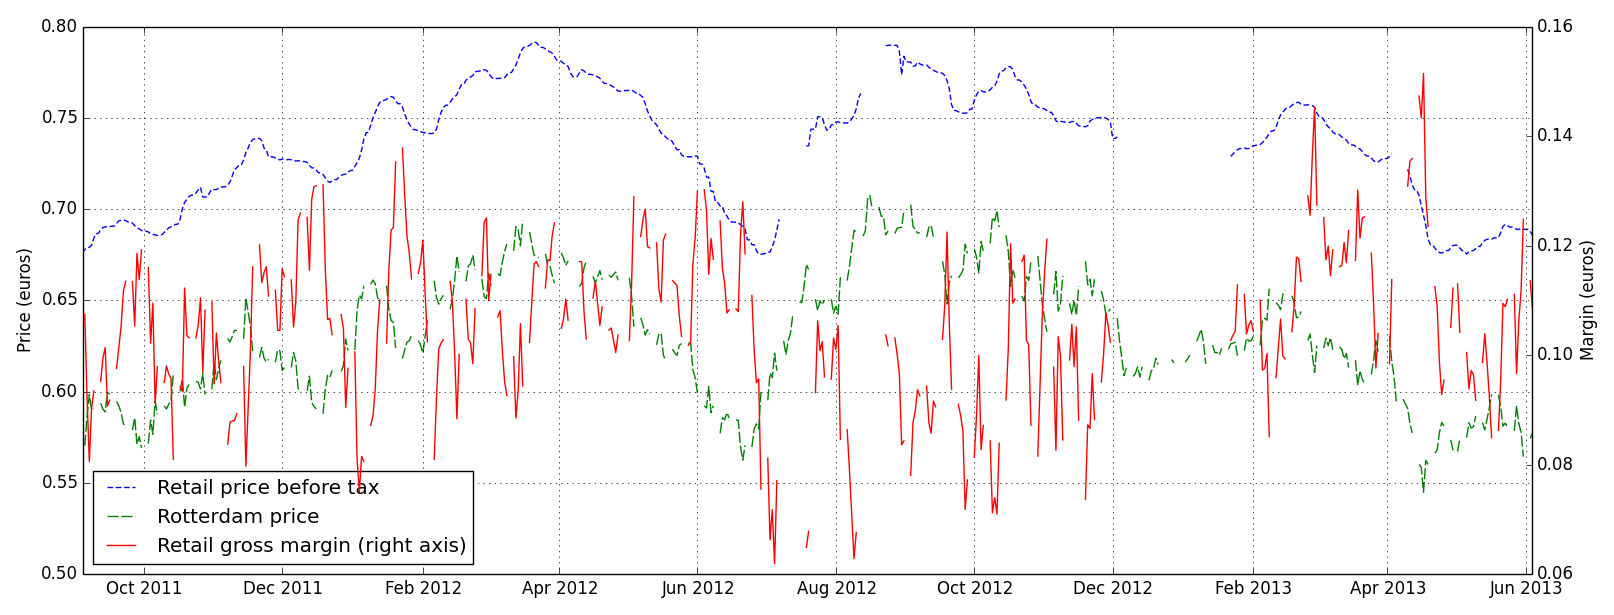
\includegraphics[width=16cm]{graphs/diesel_price_margin.png}
\end{figure}

\subsubsection{Price ridigity}

Data include prices at 9,932 gas stations in Mainland France, of which 421 are identified as highway gas stations and thus excluded from the analysis. Additionnally, 381 stations are excluded due to apparent poor data quality (less than 10 prices observed or less than a price change per month). Overall, the number of prices observed varies between 8,715 and 8,965 across days in the period studied. On average, XXX gas stations (c. XXX\% of gas stations recorded on the website) change prices within a day. On average, a gas station changes its price every XXX days.

\begin{figure}[!h]
    \caption{Daily number of price changes (09/2011-06/2012)}
	\centering
		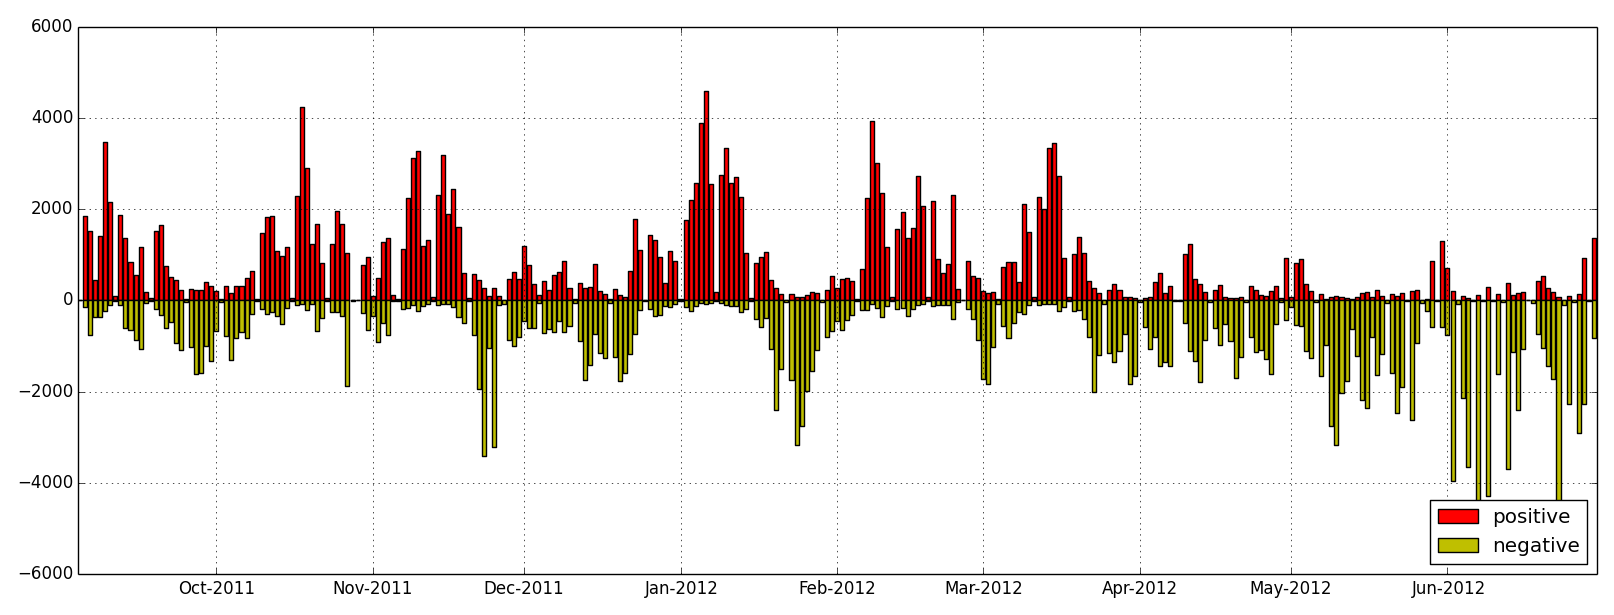
\includegraphics[width=16cm]{graphs/diesel_nb_price_chges.png}
    \floatfoot{The daily collection of prices has occasionally been delayed by a few hours resulting in some imprecision regarding the exact number of price changes occurring within one day}
\end{figure}

\subsubsection{Heterogeneity among gas stations}

Static price dispersion in French Data is easily seen in any single day price cross section. The resulting price distribution is bimodal, largely reflecting the presence of two dominant types of actors: supermarkets and oil companies. Supermarkets typically state that they use gasoline to attract consumers, while oil companies mention the quality of the service to justify higher prices. Oil companies also traditionally enjoy more demand from businesses with which they develop exclusive relationships in exchange for consumption tracking tools (firm employees pay with a specific magnetic card) and rebates. Price displayed at the gas station is then irrelevant to the transaction.

\section{Price dispersion vs. consumer information}

A simple way to measure temporal price dispersion between two stations with daily observations is to consider the probability that the station which is in general cheaper (in terms of day count) turns out to be more expensive. Formally, considering the prices $p_{it}$ and $p_{jt}$ of two stations $i$ and $j$ over $T_{ij}$ days, such that $p_{it} \ge p_{ij}$ is observed most of the time, the rank reversals statistic writes:

\begin{align*}
r_{ij} = \frac{1}{T_{ij}} \sum_{t=1}^{T_{ij}} \mathbbm{1}_{p_{jt} > p_{it}}
\end{align*}

Depending on market definitions, a database can then be built in which observations are pairs of stations assumed to compete within the same market. In the following analysis, distance as the crow flies is used with an upper distance limit of 3km (robustness checks are joined in appendix). Rank reversals are thus computed for all gas stations in the database separated by a distance of less than 3km.

A second sensitive issue which arises in the empirical analysis is the treatment of differentiation, here broadly understood as lasting differences in prices. Such an issue is traditionally addressed by working with price residuals (i.e. after taking out time and gas station fixed effects), which likely introduce errors in data. The analysis is thus performed with raw prices whenever differentiation is limited, and with residual prices when differentiation requires it.

A last issue that must be mentioned before the exposition of results is the presence in the data of significant changes in price policies. Such changes are found to be associated with a change of brand "Total" for "Total Access", the low cost brand of Total. In order to avoid spurious rank reversals (cf. appendix), all concerned pairs are excluded from the analysis. It has also been checked that no competitor's margin was affected in a different way vs. other sellers in the market whenever a change occurs.

\begin{figure}[!h]
    \caption{Percentage of rank reversals among pairs}
	\centering
		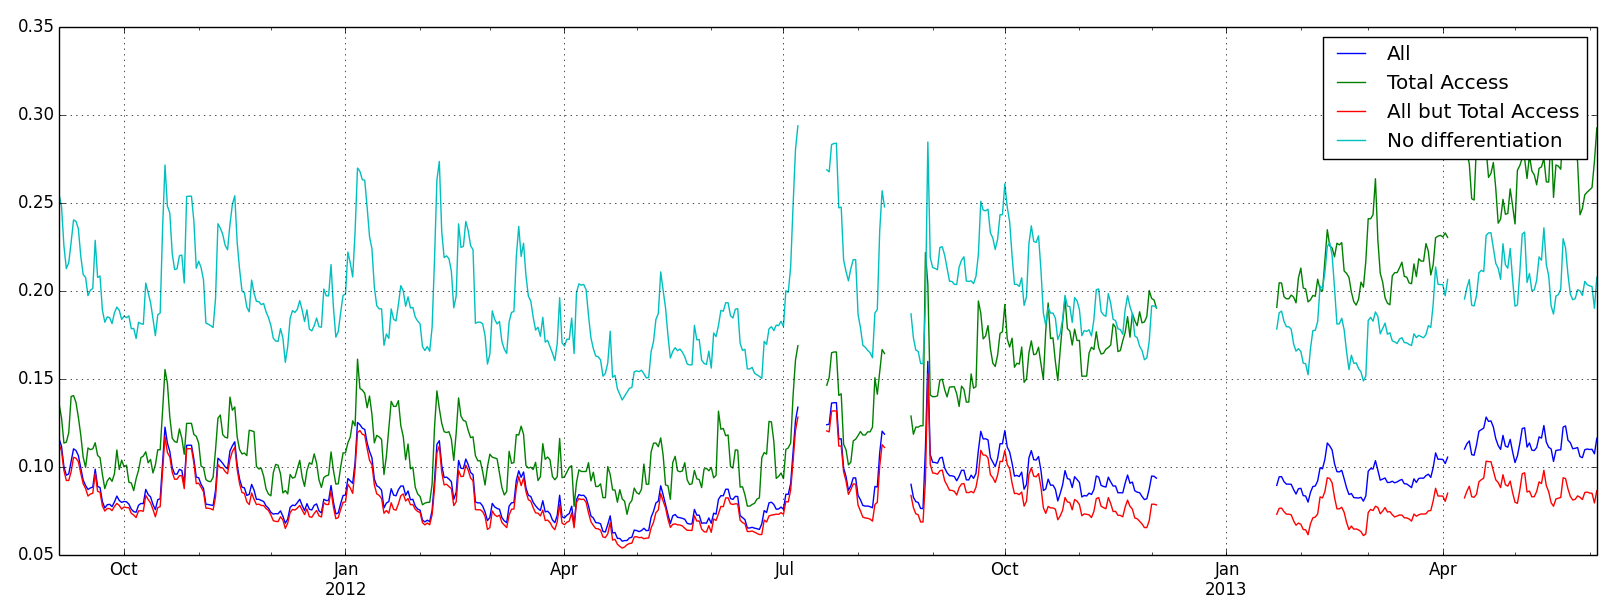
\includegraphics[width=16cm]{graphs/ecdf_rr_temporal.png}
    \floatfoot{Series represent for each day the percentage of pairs observed where the usual price order is not respected (reversed rank). No differentiation implies that pairs exhibit an average price difference below 2c/l.}
\end{figure}

Among all pairs of gas stations built with a maximum distance of 3km, the percentage of reversed pairs fluctuates between XX\% and XX\% over the period studied. The maximum of XX\% is reached at the time of the government's intervention. Figure X shows that one needs to be careful when computing rank reversals as data can be significantly biased by exogeneous factors. In the case in point, the development of "Total Access" with a change in price policy leads to measure spurious rank reversals (cf. Appendix for more details). The "No differentiation" series results from a focus on pairs which exhibit an average price difference below 2c/l.

\ \\
\begin{figure}
\caption{Pair rank reversals}
% {\renewcommand{\arraystretch}{0.8}
\centering
%\begin{center}
\begin{tabular}{lrrrrr}
\hline
{} & \multicolumn{3}{c}{Raw prices} & \multicolumn{2}{c}{Residual prices}  \\
{} & All & No Total & Price difference & Price difference & Price difference \\
{} & {} & Access & $\le$ 2c/l (mean) & $\le$ 2c/l (mean) & $\ge$ 2c/l (mean)\\
\hline
Max $d_{ij}$: 3km & {} & {} & {} & {} & {} \\
\hline
Nb pairs & 16,142 & 13,846 & 5,166 & 5,166 & 8,680 \\
Mean & 0.09 & 0.08 & 0.19 & 0.39 & 0.45 \\
Std & 0.13 & 0.12 & 0.13 & 0.11 & 0.05 \\
Median & 0.02 & 0.01 & 0.17 & 0.43 & 0.46 \\
\hline
Max $d_{ij}$: 5 km & {} & {} & {} & {} & {} \\
\hline
Nb pairs & 33,478 & 28,433 & 10,314 & 10,314 & 18,119 \\
Mean & 0.09 & 0.08 & 0.21 & 0.41 & 0.45 \\
Std & 0.13 & 0.12 & 0.13 & 0.10 & 0.04 \\
Median & 0.02 & 0.01 & 0.19 & 044 & 0.46 \\
\hline
\multicolumn{6}{l}{\small Pairs including a Total Access gas station are excluded in the three last columns}\\
\end{tabular}
%\end{center}
\end{figure}

A clear ranking of empirical distribution functions of rank reversals can be observed among pairs of gas stations depending on distances. This is consistent with the idea that nearby gas stations compete in a (virtually) complete information setting, where there is no particular reason to expect rank reversals. Conversely, distance can create an information issue for other pairs, leading to the inexistence of an equilibrium in pure strategies.

\begin{figure}[H]
\centering
\caption{Empirical distribution functions of rank reversals (raw prices)}
\begin{subfigure}{.4\linewidth}
\centering
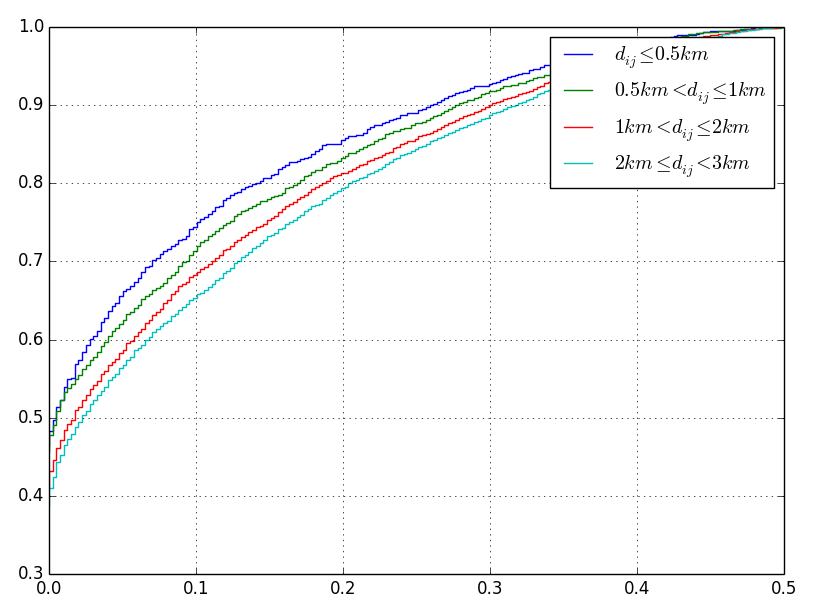
\includegraphics[width=6cm]{graphs/ecdf_rr_all.png}
\caption[short]{All pairs}
\end{subfigure}
\begin{subfigure}{.4\linewidth}
\centering
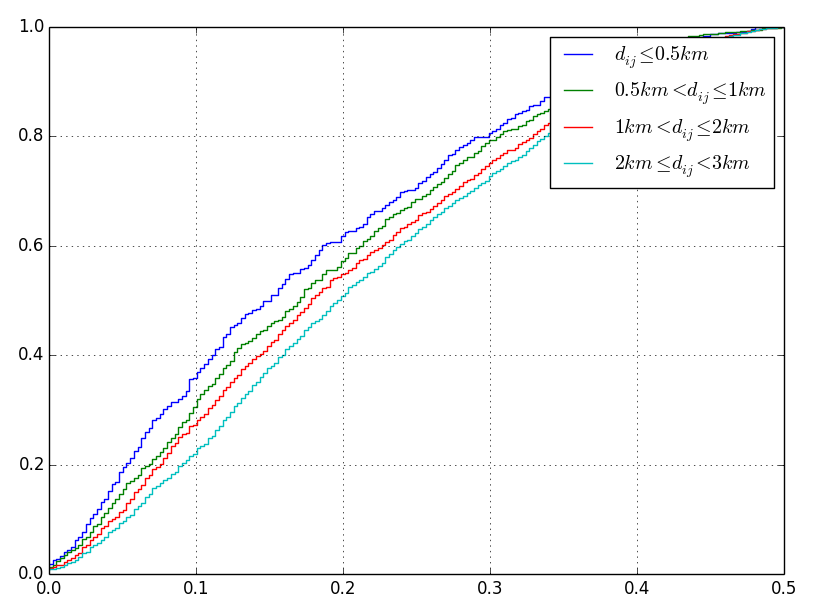
\includegraphics[width=6cm]{graphs/ecdf_rr_nodiff.png}
\caption[short]{Pairs with low differentiation}
\end{subfigure}
\end{figure}

In order to evaluate the hypothesis according to which information is connected to price dispersion, two measures of price dispersion: rank reversals and standard deviation in spread, are regressed on a proxy for consumer information: distance between stations.

\begin{table}[h]\centering
\def\sym#1{\ifmmode^{#1}\else\(^{#1}\)\fi}
\caption{Regression of rank reversals}
\begin{tabular}{lccc}
\hline
\hline
{} & No differentiation & No differentiation & Differentiation \\
{} & raw prices & residual prices & residual prices \\
\hline
OLS: distance             &  0.014\sym{***}  &  0.020\sym{***}  &  0.001\sym{}\\
{}                        & (0.002)          & (0.002)          & (0.001)   \\
OLS: dummy                & -0.024\sym{***}  & -0.034\sym{***}  & -0.006\sym{***}\\
{}                        & (0.007)          & (0.006)          & (0.002) \\
Quantile 0.25: dummy      & -0.027\sym{***}  & -0.067\sym{***}  & -0.007\sym{***}\\
{}                        & (0.008)          & (0.010)          & (0.003)  \\
Quantile 0.50: dummy      & -0.024\sym{*}    & -0.030\sym{***}  & -0.007\sym{**}\\
{}                        & (0.011)          & (0.005)          & (0.002)    \\
Quantile 0.75: dummy      & -0.027\sym{*}    & -0.007\sym{*}    & -0.002\sym{}\\
{}                        & (0.014)          & (0.003)          & (0.001)   \\
\hline
N                         & 4,183            &   4,183          &     8,312    \\
\hline\hline
\multicolumn{4}{l}{\footnotesize Standard errors in parentheses}\\
\multicolumn{4}{l}{\footnotesize \sym{*} \(p<0.05\), \sym{**} \(p<0.01\), \sym{***} \(p<0.001\)}\\
\end{tabular}
\end{table}

Using maximum 1km and 2km allows to build databases containing respectively X and X pairs of gas stations. As expected, rank reversals between two stations decreases in the average spread between their prices, with a large number exhibiting no rank reversals. In order to reduce the influence of static dispersion, the sample is subset based on the value of the average spread between prices. Results are presented for a maximum average spread of 0.02c/l i.e. a 1\% to 2\% average difference in prices. Finally, a last element is taken in consideration: the conversion of XXX gas stations by the brand Total to low cost gas stations, which generates a large number of spurious rank reversals.

Statistics provided in \cite{TAP11} to describe prices and mark up suggest that the issue of static price dispersion is not severe. In all pairs obtained with a 1 mile maximum distance between stations, depending on fuel type, average spread amounts to 1\% to 2\% of average price, over 90\% of pairs exhibit positive rank reversals, and the average pair rank reversals varies between c.12\% and c.15\%. Results do not vary significantly with a 2 mile maximum distance. Static price dispersion can therefore arguably be neglected, thus avoiding the shortcomings associated with price cleaning.

\section{Market price dispersion}

While the emphasis has so far been laid on examining empirical evidence about the link between price dispersion and consumer information, the following section seeks to compare predictions from a model a la \cite{VAR80} with French retail gasoline market data.

The methodology employed by \cite{TAP11} consists in considering each gas station successively as the center of a market delimited by a circle of a given radius (robustness of results to variations in radius size is checked). Various statistics accounting for price dispersion can then be computed for each market and period. If one observes $N$ stations close to each other (e.g. with a limit radius of 2km: if no two stations are separated by a distance of more than 2 km) and with prices posted over $T$ periods, this will result in $N*T$ observations as each station is successively considered and, for each station, a statistic representing price dispersion is computed at each period. An expected consequence is that it tends to over represent markets with higher gas station density (typically cities).

Regressions are then run using raw prices and cleaned prices. Also, in order to address the issue of overlapping markets, regression are performed on dispersion data generated in a way that prevents market overlap (the precise metholody is not given?). Descriptive statistics performed on raw prices are provided.

Standard market dispersion statistics such as range and standard deviation are strongly influenced by static price dispersion. As a consequence, contrarily to the previous section where descriptives statistics performed on raw prices arguably provided a most conservative first idea of price dispersion, clean prices are now to be preferred despite their shortcomings. Results are reported with clean prices, raw prices for markets obtained with radiuses of respectively 3 and 5km. Additionnally, results are reported for non overlapping markets built in a way that is detailed in appendix.

\begin{figure}[h]
\caption{Overview of market price dispersion}
% {\renewcommand{\arraystretch}{0.8}
\begin{center}
\begin{tabular}{lrrr}
\hline
{} & Radius 5km & Radius 3km & No overlap\\
\hline
Nb of markets & 6794 & 5614 & 386 \\
Avg nb competitors & 11.2 & 6.7 & 3.9 \\
\hline
Raw prices & & & \\
\hline
Market price range & 0.116 & 0.105 & 0.089\\
Market gain from search & 0.046 & 0.044 & 0.036 \\
Market price std & 0.046 & 0.045 & 0.045 \\
\hline
Residual prices & & & \\
\hline
Market price range & 0.033  & 0.028 & 0.020 \\
Market gain from search & 0.017 & 0.014 & 0.010 \\
Market price std & 0.011 & 0.011 & 0.010 \\
\hline
\end{tabular}
\end{center}
\floatfoot{Each statistic accounting for price dispersion is first computed for each local market across time. The table reports averages across markets. At the market level, price dispersion has been computed only for days when more than two thirds of competitors' prices were available. Only markets with more than 50 days of data are then taken into account to compute reported statistics.}
\end{figure}

In \cite{TAP11}, the number of rivals within 2 miles (c.3.2km) of each station is rather similar in all states: from 13.38 in New Jersey to 14.22 in Texas (resp. 4.25 to 4.74 with 1 mile). The average distance to the closest rival ranges from 0.38 to 0.49 miles (c. 600 to 800m).

\begin{table}[htbp]\centering
\def\sym#1{\ifmmode^{#1}\else\(^{#1}\)\fi}
\caption{Regressions of market dispersion}
\begin{tabular}{lcccc }
\hline
\hline
{} & All & All & No overlap & Stable markets\\
{} & Raw prices & Residual prices & Residual prices &  Residual prices \\
\hline
Gains from search & & & & \\
\hline
Nb competitors           &  0.003\sym{***}  &  0.001\sym{***}  &  0.001\sym{***}  & 0.001\sym{***} \\
{}                       & (0.000)          & (0.000)          & (0.000)          & (0.000)        \\
Cost                     &  0.007\sym{*  }  & -0.006\sym{*}    & -0.005\sym{}     & -0.005\sym{}   \\
{}                       & (0.003)          & (0.003)          & (0.003)          & (0.003)        \\
Intercept                &  0.015\sym{***}  &  0.015\sym{***}  & 0.013\sym{***}   &  0.012\sym{**} \\
{}                       & (0.004)          & (0.004)          & (0.004)          & (0.004)        \\
\hline
Standard deviation & & & & \\
\hline
Nb competitors           &  0.000\sym{***}  &  0.000\sym{***}  &  0.000\sym{***}  &  0.000\sym{}          \\
{}                       & (0.000)          & (0.000)          & (0.000)          & (0.000)    \\
Cost                     & -0.001\sym{   }  & -0.009\sym{***}  & -0.009\sym{***}  & -0.008\sym{***} \\
{}                       & (0.002)          & (0.002)          & (0.002)          & (0.003)         \\
Intercept                &  0.044\sym{***}  &  0.022\sym{***}  &  0.021\sym{***}  &  0.021\sym{***} \\
{}                       & (0.003)          & (0.003)          & (0.003)          & (0.004)    \\
\hline
Coefficient of variation & & & & \\
\hline
Nb competitors           &  0.000\sym{***}  &        \sym{}    &       \sym{}     &\\
{}                       & (0.000)          &                  &                  &\\
Cost                     & -0.024\sym{***}  &        \sym{}    &       \sym{}     &\\
{}                       & (0.001)          &                  &                  &\\
Intercept                &  0.064\sym{***}  &        \sym{}    &       \sym{}     &\\
{}                       & (0.002)          &                  &                  &\\
\hline
Range & & & & \\
\hline
Nb competitors           &  0.006\sym{***}  &  0.002\sym{***}  &  0.003\sym{***}  &  0.002\sym{***} \\
{}                       & (0.000)          & (0.000)          & (0.000)          & (0.000)         \\
Cost                     & -0.004\sym{}     & -0.025\sym{***}  & -0.021\sym{***}  & -0.019\sym{***} \\
{}                       & (0.005)          & (0.005)          & (0.005)          & (0.006)         \\
Intercept                &  0.074\sym{***}  & 0.048\sym{***}   &  0.041\sym{***}  &  0.038\sym{***} \\
{}                       & (0.007)          & (0.007)          & (0.007)          & (0.008)         \\
\hline
N                        & 2,756,096        & 2,756,096        & 493,356          &\\
\hline\hline
\multicolumn{4}{l}{\footnotesize Standard errors in parentheses}\\
\multicolumn{4}{l}{\footnotesize \sym{*} \(p<0.05\), \sym{**} \(p<0.01\), \sym{***} \(p<0.001\)}\\
\end{tabular}
\end{table}

Estimation results show that dispersion is increasing in the number of firm and decreasing in price.

\section{Conclusion}

\newpage

\bibliography{references}

\newpage

\appendix

\section{Additionnal regression results}

\begin{table}[htbp]\centering
\def\sym#1{\ifmmode^{#1}\else\(^{#1}\)\fi}
\caption{Regression of standard deviation in spread}
\begin{tabular}{lrrr}
\hline
\hline
{} & No differentiation & No differentiation & Differentiation \\
{} & raw prices & residual prices & residual prices \\
\hline
OLS: distance &  0.001 \sym{***}&      0.001\sym{***}&       0.000\sym{***}\\
{} &     (0.000)         &     (0.000)         &     (0.000)   \\
OLS: dummy &  -0.001\sym{***}&      -0.001\sym{***}&     -0.001\sym{***}\\
{} &    (0.000)     &     (0.000)         &     (0.000) \\
Quantile 0.25: dummy     &       -0.001\sym{**}&       -0.001\sym{**}&       -0.000\sym{}\\
{} &     (0.000)       &     (0.000)         &     (0.000)  \\
Quantile 0.50: dummy     &       -0.001\sym{**}&      -0.001\sym{*}&       -0.000\sym{}\\
{} &  (0.000)         &     (0.000)         &     (0.000)    \\
Quantile 0.75: dummy     &       -0.001\sym{**}&     -0.001\sym{**}&       -0.000\sym{}\\
{} &     (0.001)         &     (0.001)         &     (0.000)   \\
\hline
N      &     4,183         &     4,183      &     8,312    \\
\hline\hline
\multicolumn{4}{l}{\footnotesize Standard errors in parentheses}\\
\multicolumn{4}{l}{\footnotesize \sym{*} \(p<0.05\), \sym{**} \(p<0.01\), \sym{***} \(p<0.001\)}\\
\end{tabular}
\end{table}

\section{Consumer search vs. price levels and dispersion}

Zagaz.com and Prix-carburant.gouv.fr offer the opportunity to observe trend in user registrations and/or trafic. Such information can then be merged with price data to study the relation between proxies for consumer search efforts and price levels or dispersion.

\end{document}
